\documentclass[11pt,a4paper]{article}
\usepackage[T1]{fontenc}
\usepackage{lmodern}
\usepackage[margin=20mm]{geometry}
\usepackage{graphicx,float,booktabs,caption,listings,titlesec,hyperref}
\hypersetup{hidelinks,pdftitle={DT081A Laboratory 1 - Individual Report Draft},
  pdfauthor={Yacoub Dawli}}
\graphicspath{{../figures/}}
\setlength{\parindent}{0pt}
\setlength{\parskip}{2pt}
\setlength{\textfloatsep}{6pt}
\setlength{\intextsep}{5pt}
\titleformat{\section}{\large\bfseries}{\thesection}{0.6em}{}
\titleformat{\subsection}{\normalsize\bfseries}{\thesubsection}{0.6em}{}
\titlespacing*{\section}{0pt}{6pt}{3pt}
\titlespacing*{\subsection}{0pt}{5pt}{2pt}
\captionsetup{font=small,labelfont=bf,skip=3pt}
\lstset{basicstyle=\ttfamily\fontsize{8.5}{10}\selectfont,
  columns=fullflexible,keepspaces=true,showstringspaces=false,
  aboveskip=1pt,belowskip=2pt}
\emergencystretch=1em
\clubpenalty=10000
\widowpenalty=10000
\raggedbottom
\pagestyle{plain}

\begin{document}
\fontsize{10.5}{12.5}\selectfont
\begin{center}
{\large DT081A - Signal and Image Processing}\\[2pt]
{\Large\bfseries Laboratory 1 Report}\\[3pt]
Yacoub Dawli \quad \href{mailto:yada2100@student.miun.se}{\texttt{yada2100@student.miun.se}}\\[2pt]
2026-10-29
\end{center}
\vspace{-5pt}

\section{Introduction}
This lab explored signal generation, Fourier analysis, sampling, image
resampling, quantization, quality measurements and noise reduction. Audio
analysis also demonstrated aliasing.

\section{Experimental Setup}
I used Python, NumPy, SciPy, Matplotlib, Pillow and scikit-image, following the
teacher's Lab 1 examples. Inputs were Lenna, four course TIFF images, and piano,
rain and speech recordings. Noise used seed 2026.

\section{Results and Analysis}
% Teacher 1.1 Q1-Q5.
\subsection{Signal Generation and Visualization}
The signals were a 10 Hz sine, 5 Hz square and 5 Hz sawtooth.
The sawtooth \(2((5t)\bmod 1)-1\) makes rising ramps from \(-1\) towards \(+1\).
Changing the sine to 20 Hz doubled its cycle count.
The sign and ceil expressions differed only at \(t=0\): 0 versus \(-1\).
Ceil did not extend the positive part.
At an exact sine value of \(-1\), ceil would instead give \(-3\).
Adding the sine and square gave jumps and curves, a range near \(-2\) to \(+2\),
and a 0.2 s period. Synthesizers use waveform shape to change sound.

% Teacher 1.2 Q1-Q5.
\subsection{Fourier Transform and Frequency Analysis}
The 10 and 20 Hz components had amplitudes 1 and 0.5. Their FFT peaks were at
9.990 and 19.980 Hz. Adding 30 Hz at amplitude 0.25 gave a smaller
29.970 Hz peak. The endpoint-including grid has spacing \(1/999\) s, explaining
the offsets. Noise of standard deviation 0.2 raised
the spectral background, while the main peaks remained visible.

The chirp phase was \(2\pi(10t+20t^2)\), giving \(f(t)=10+40t\): 10--50 Hz in
one second. Its cycles became closer together, and its whole-signal FFT spread
across a frequency range. Figure~\ref{fig:chirp} shows the rising band.
The 256-sample STFT used \(10\log_{10}|Z|^2\) for power in dB.
Audio equalizers use frequency analysis to change selected bands.

\begin{figure}[H]
\centering
% Saved spectrogram panel; trims are in PDF points. Source PNG is unchanged.
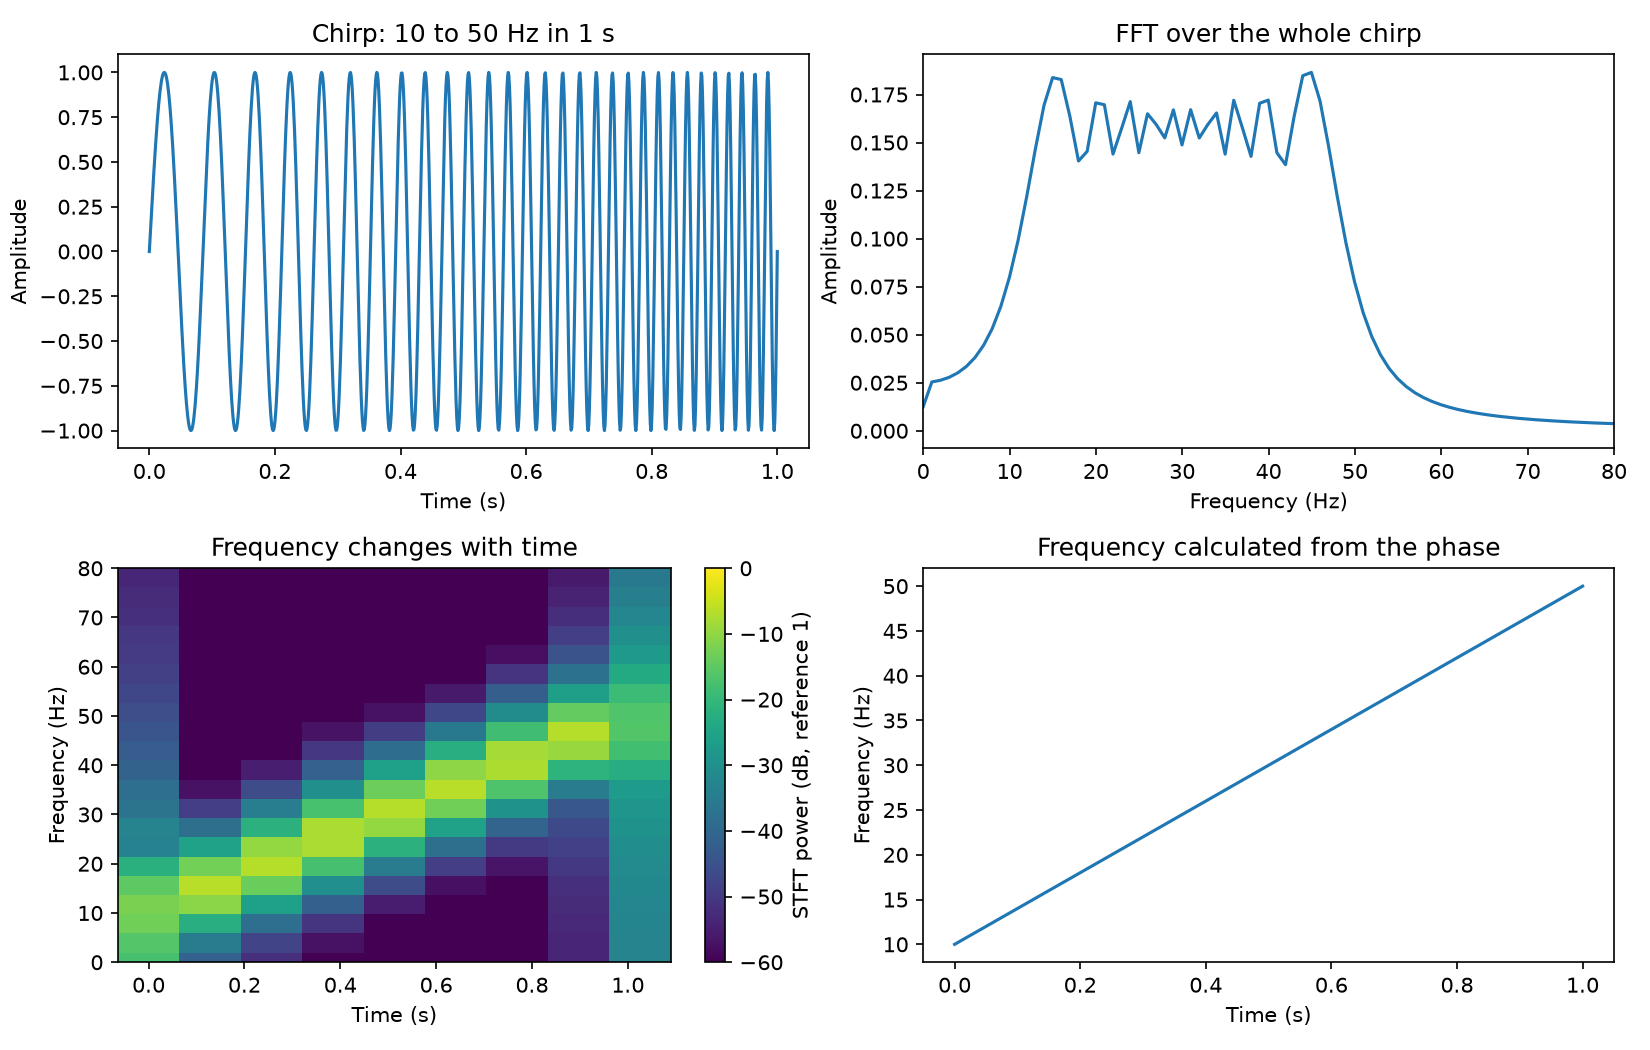
\includegraphics[trim=0 0 396bp 252bp,clip,width=108mm]{chirp.png}
\caption{The chirp's frequency increases with time. Colour shows STFT power.}
\label{fig:chirp}
\end{figure}

% Teacher 1.3 Q1-Q5.
\subsection{Sampling and Aliasing}
The Nyquist rate is twice the signal frequency (Table~\ref{tab:sampling}).
Sampling 10 Hz at 25 Hz avoided folding; sampling 20 Hz at 30 Hz gave a 10 Hz
alias. Signed matches \(-5\), \(-10\) and \(-1\) Hz describe reversed phase
progression. The 10 Hz/11 Hz case explains slow or reverse wagon-wheel motion.
In photography, undersampled repeating detail can create false moire patterns.

\begin{table}[H]
\centering
\caption{Sampling results. Positive alias magnitudes are listed.}
\label{tab:sampling}
\small
\begin{tabular}{rrrr}
\toprule
Signal (Hz) & Sampling rate (Hz) & Nyquist rate (Hz) & Alias (Hz)\\
\midrule
10 & 15 & 20 & 5\\
10 & 25 & 20 & 10, no aliasing\\
20 & 30 & 40 & 10\\
10 & 11 & 20 & 1\\
\bottomrule
\end{tabular}
\end{table}

% Teacher 2.1 Q1-Q6.
\subsection{Image Resampling and Requantization}
The grayscale image had \(512\times512\) pixels. Simple resampling kept
every nth pixel and repeated it to full size. Factor 2 changed fine edges;
factor 4 showed clear blocks, and factor 8 was worse. Requantization
reduced grey levels, causing bands rather than blocks
(Figure~\ref{fig:images}). At this size, 6 bpp looked close to the
original; 4 bpp showed clear bands and 2 bpp strong bands. These allow 64, 16
and 4 levels respectively. Visibility depends on the image and viewer.

\begin{figure}[H]
\centering
\begin{minipage}[b]{0.31\linewidth}
\centering\small Original\\[2pt]
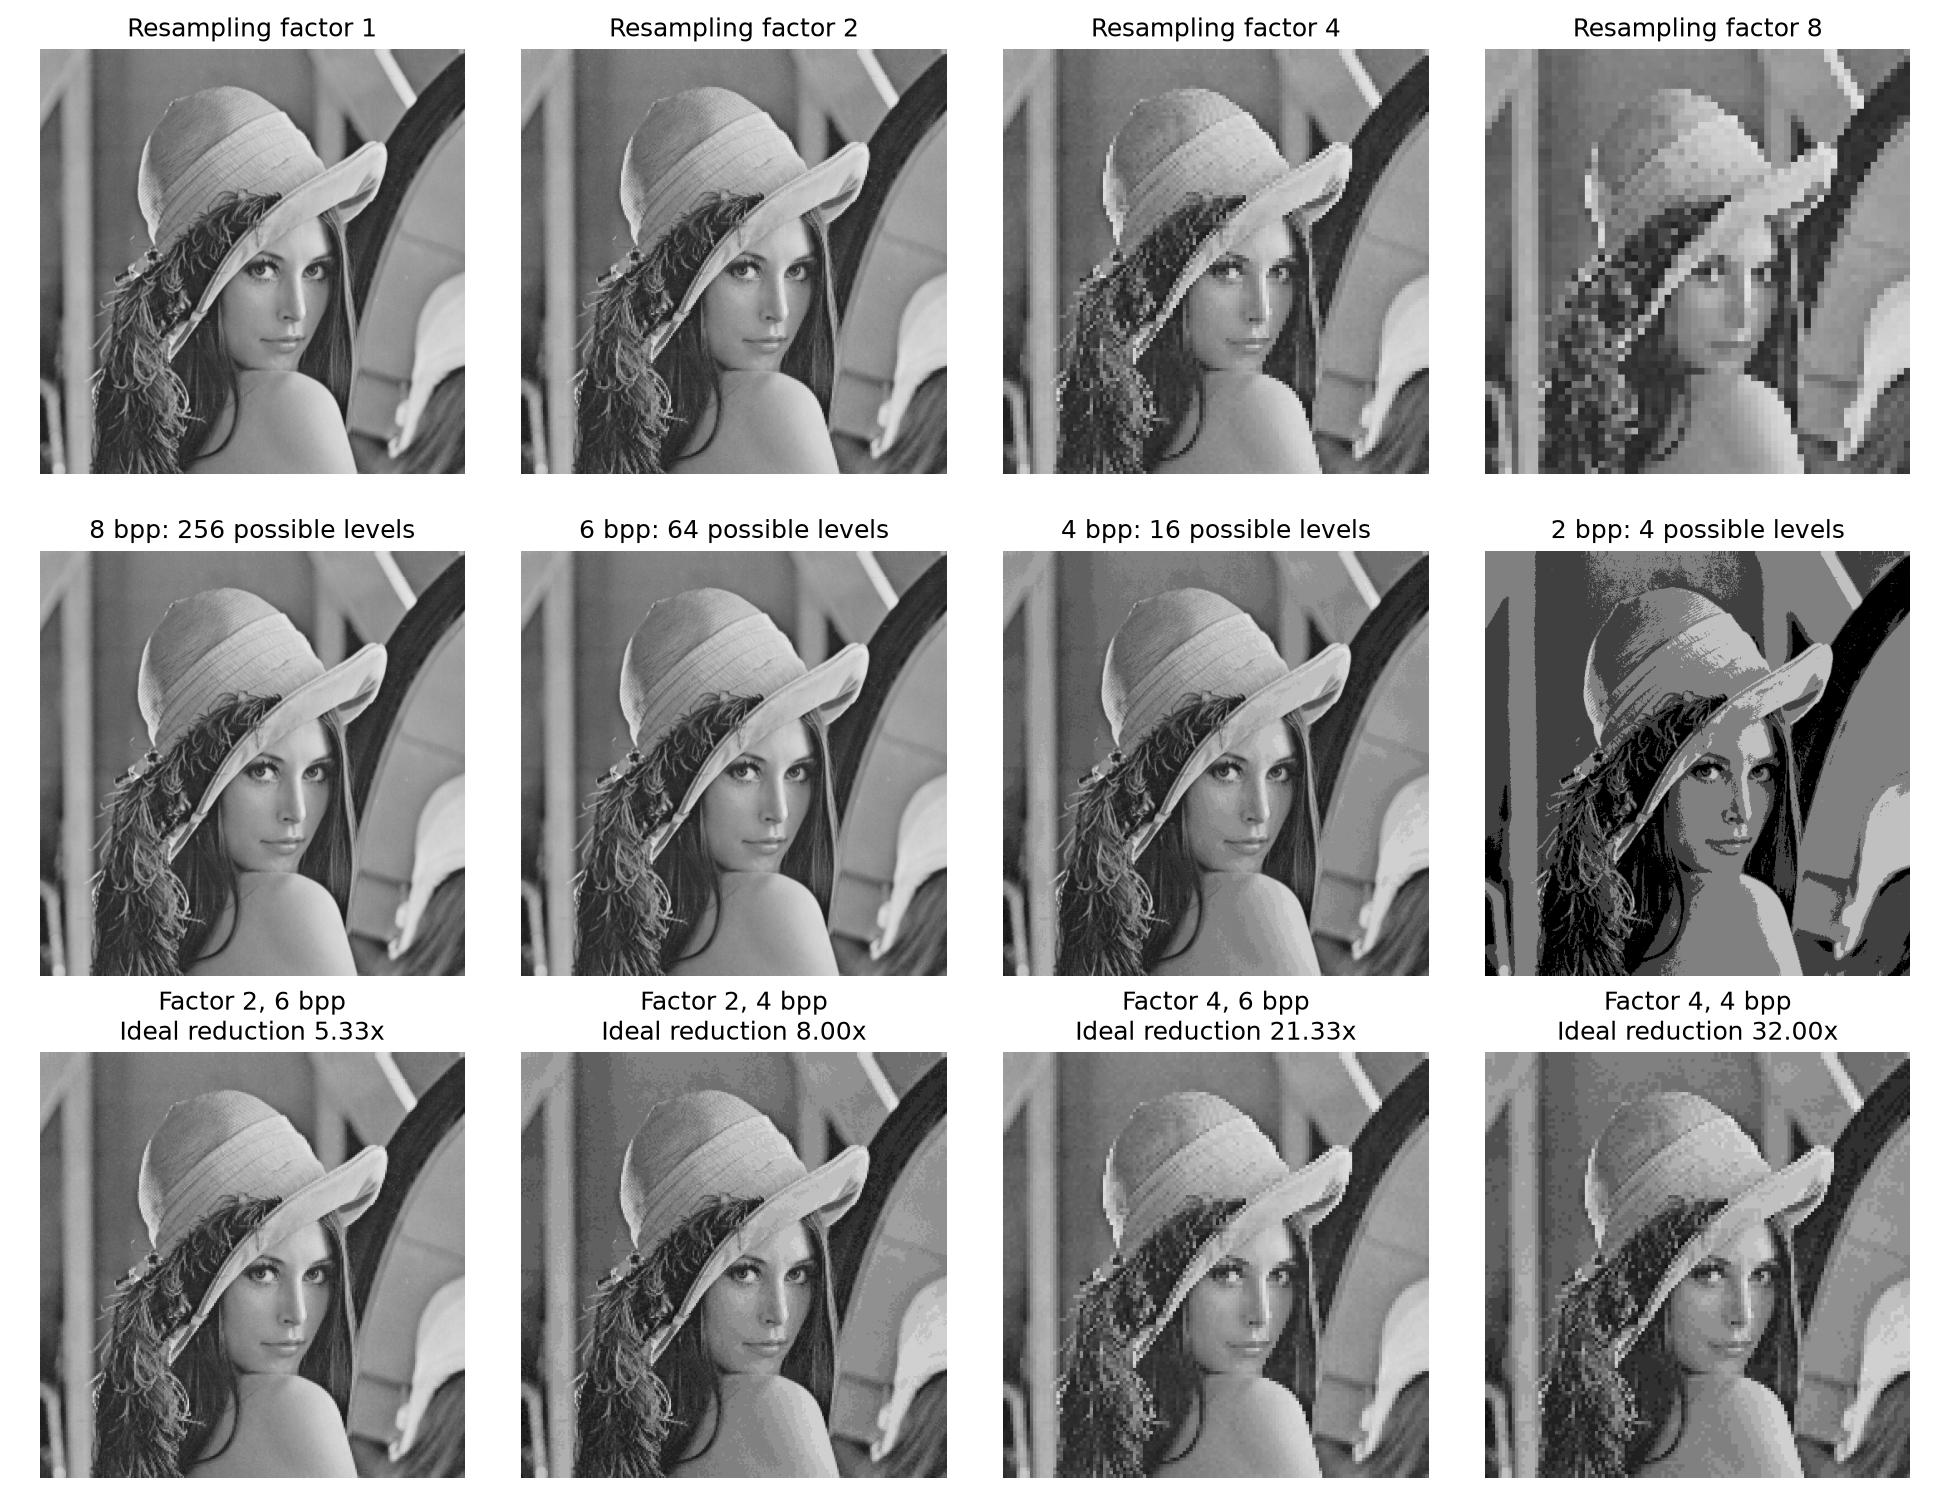
\includegraphics[trim=19.2bp 492.48bp 712.8bp 23.52bp,clip,width=\linewidth]{image_sampling_quantization.png}
\end{minipage}\hfill
\begin{minipage}[b]{0.31\linewidth}
\centering\small Resampling, factor 4\\[2pt]
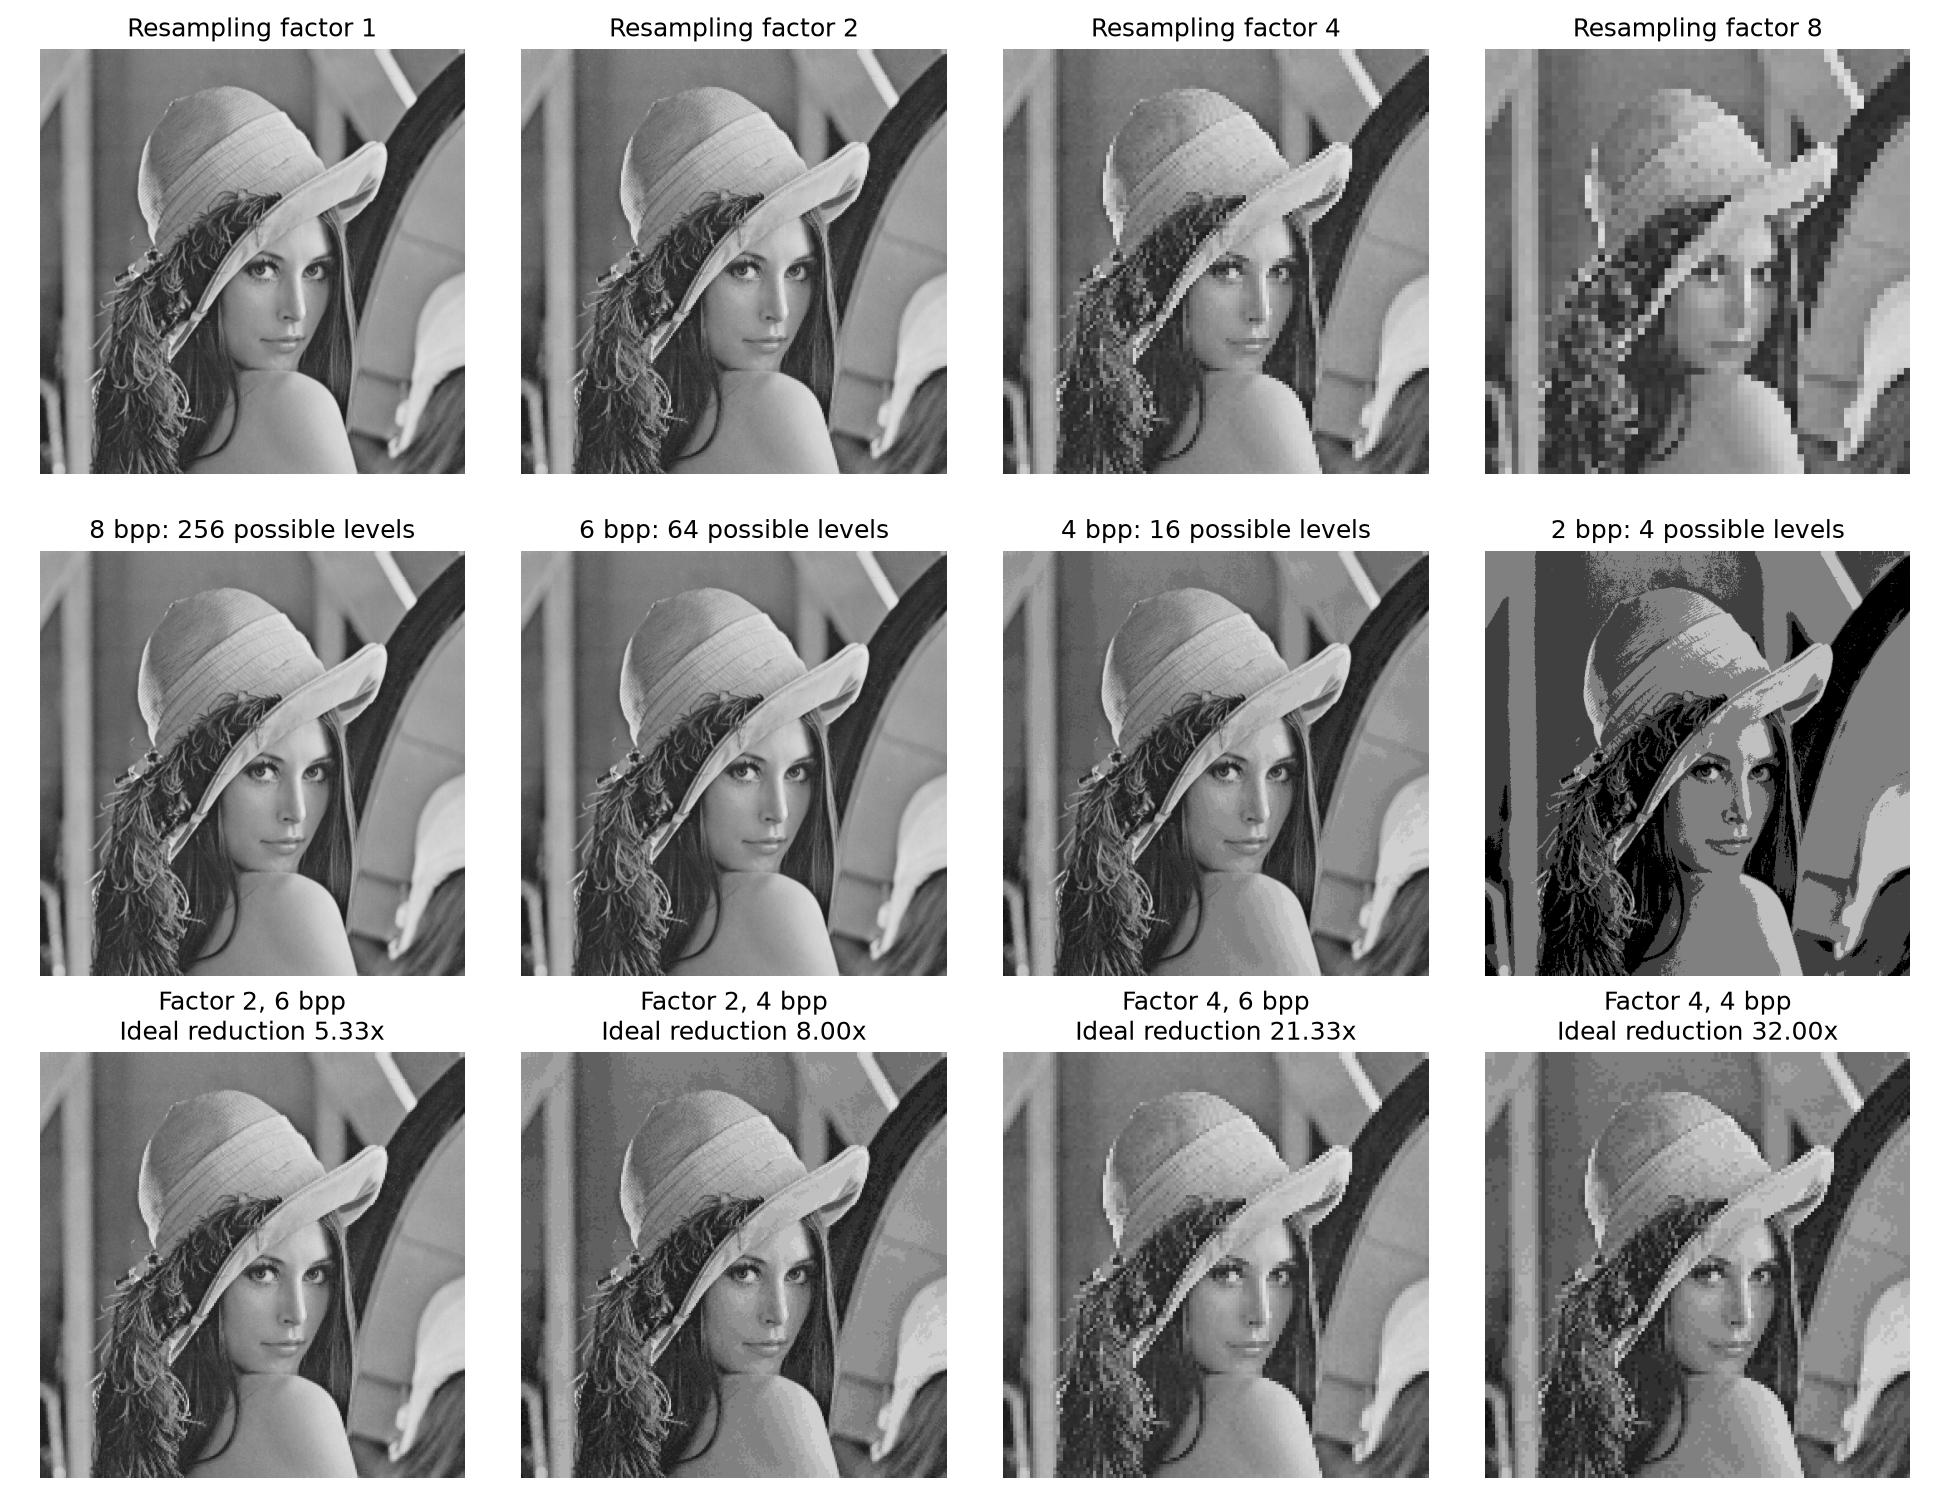
\includegraphics[trim=481.44bp 492.48bp 250.08bp 23.52bp,clip,width=\linewidth]{image_sampling_quantization.png}
\end{minipage}\hfill
\begin{minipage}[b]{0.31\linewidth}
\centering\small Requantization, 4 bpp\\[2pt]
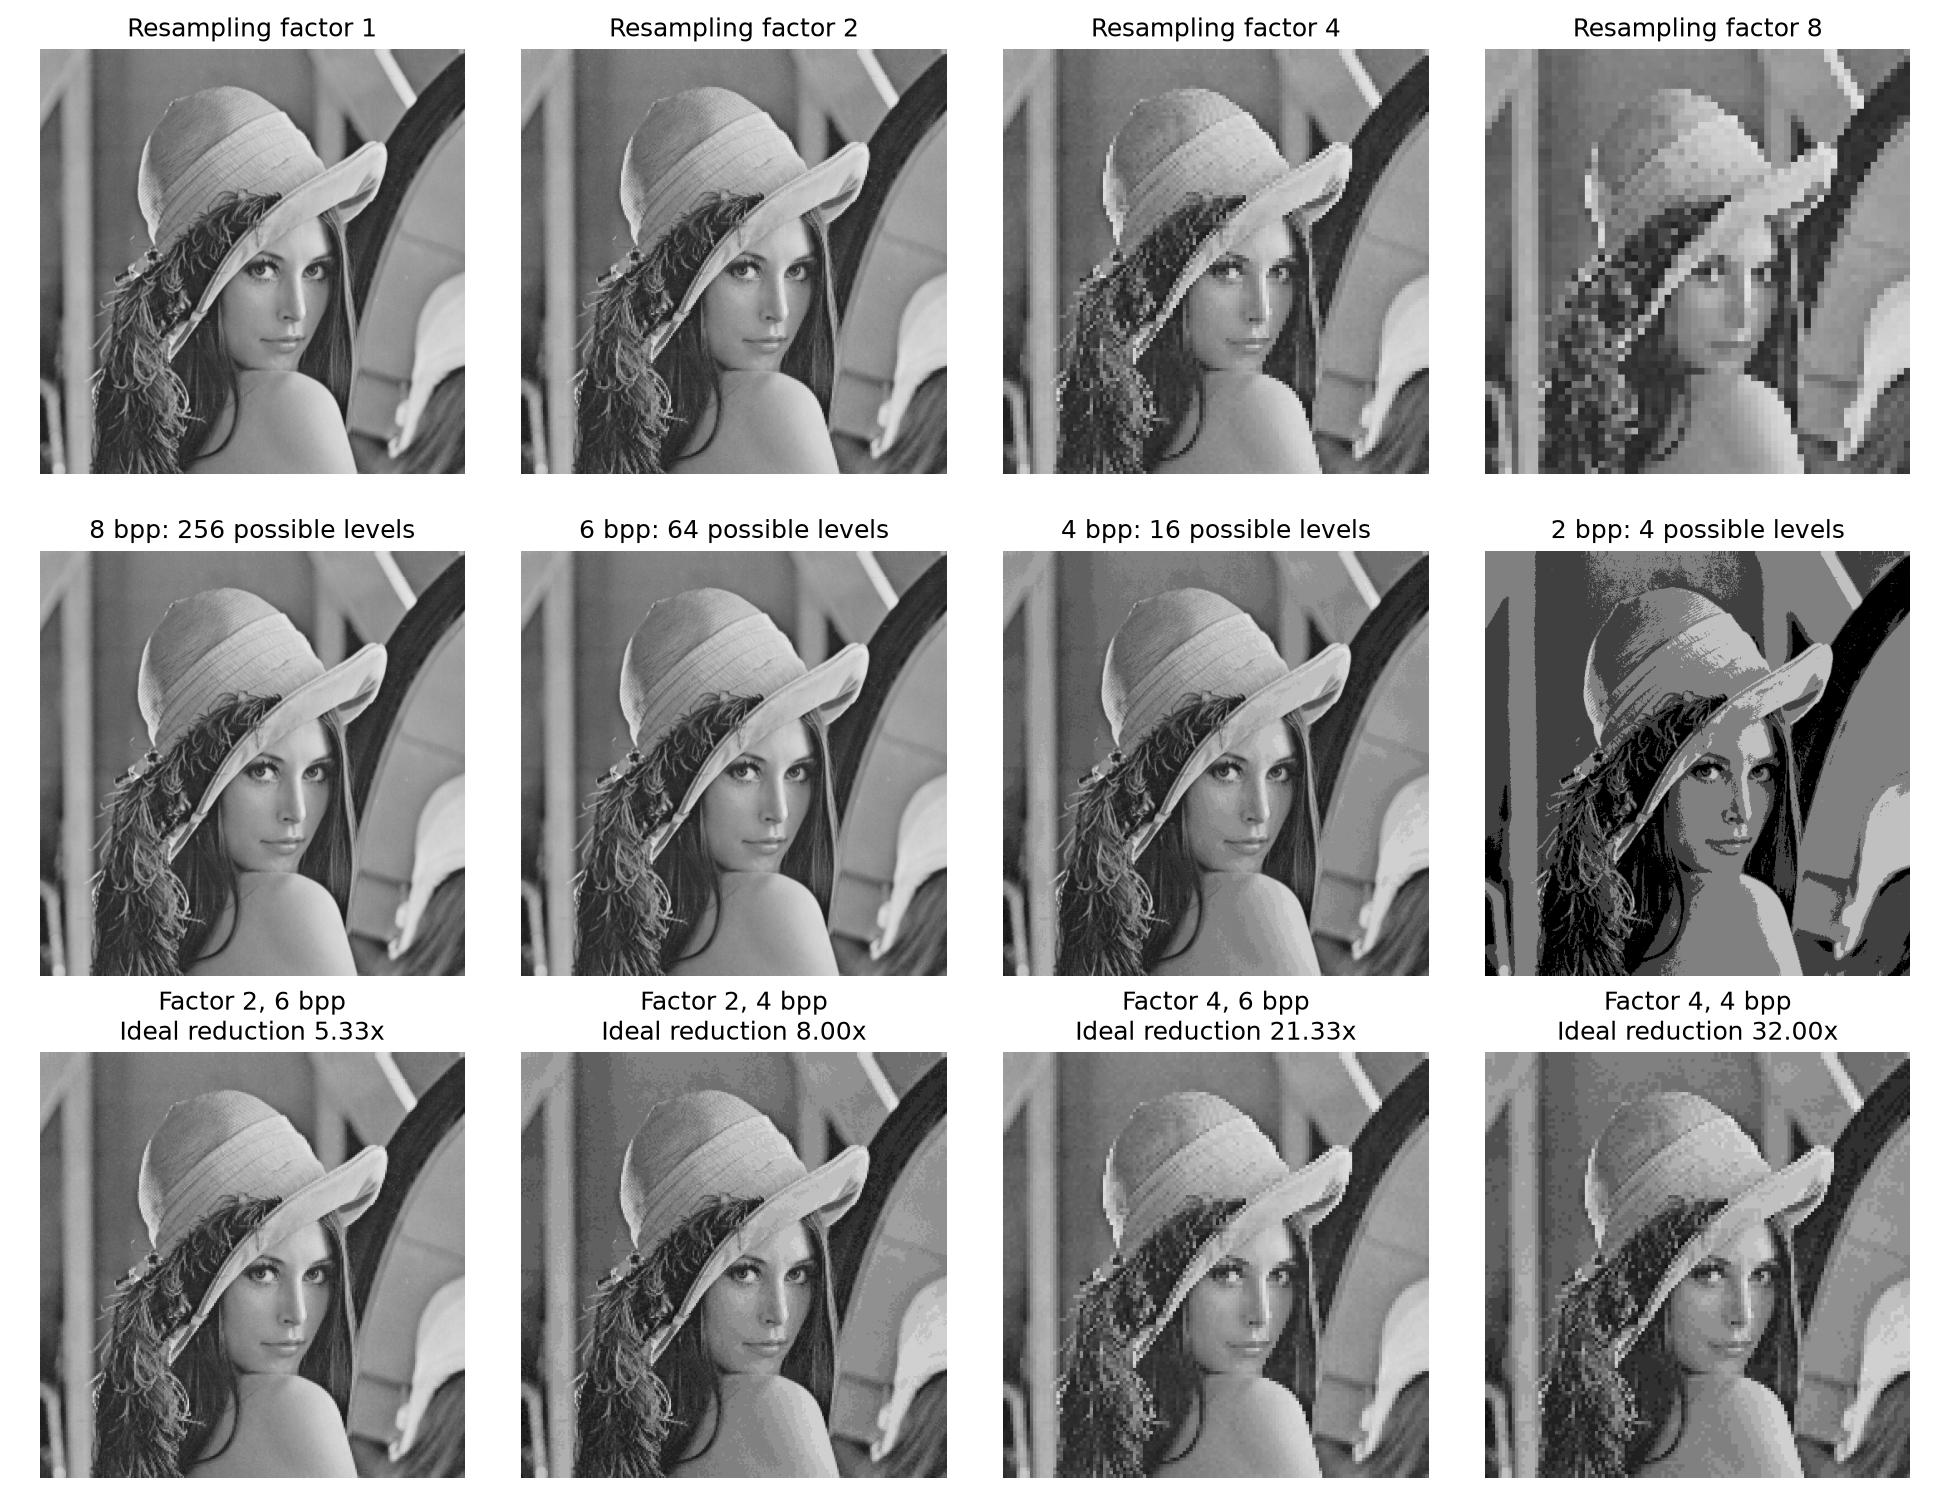
\includegraphics[trim=481.44bp 251.52bp 250.08bp 264.48bp,clip,width=\linewidth]{image_sampling_quantization.png}
\end{minipage}
\caption{Resampling loses detail; requantization creates bands. All panels use grey levels 0--255.}
\label{fig:images}
\end{figure}

The combined operation resampled and then requantized. Factor 2 with 6 bpp
was my best balance; factor 4 reduced more but looked blockier
(Table~\ref{tab:images}). For factor \(n\) and bit depth \(b\), the ideal ratio is
\(8n^2/b\), assuming packed reduced pixels from an 8 bpp original and excluding
headers. The expanded NumPy arrays
are not compressed files.

For a fair comparison, both simple and bicubic methods reduced each dimension
by four and reconstructed to \(512\times512\). Pillow bicubic resizing looked
smoother, although fine detail softened. Its higher PSNR agrees with this result.
One run took 1.504 ms for simple resampling and 4.181 ms for bicubic.
Bicubic does more calculation; timings vary.

Resampling lost portrait texture, grass detail and small aerial features.
Bicubic reduced block edges but could not restore everything. Requantization
kept much texture, while smooth areas showed bands, especially on peppers.

% Teacher 2.2 Q1-Q5.
\subsection{PSNR and SSIM}
PSNR used \(10\log_{10}(255^2/\mathrm{MSE})\), with floating-point subtraction
before squaring. Table~\ref{tab:images} shows more pixel error after resampling
than after requantization. The requantized image also looked closer to the
original, so the PSNR ranking agreed with this comparison.

\begin{table}[H]
\centering
\caption{Image quality and selected ideal reductions. A dash means not listed.}
\label{tab:images}
\small
\begin{tabular}{lrrr}
\toprule
Processing & Ideal reduction & PSNR (dB) & SSIM\\
\midrule
Simple resampling, factor 4 & --- & 22.71 & 0.6589\\
Requantization, 4 bpp & --- & 29.21 & 0.8832\\
Factor 2, 6 bpp & \(5.33\times\) & 28.14 & ---\\
Factor 4, 6 bpp & \(21.33\times\) & 22.66 & ---\\
Bicubic, factor 4 & --- & 28.84 & ---\\
\bottomrule
\end{tabular}
\end{table}

The parameter sweep covered factors 1, 2, 4 and 8 at 1--8 bpp. Higher bit depths
improved quality, but resampled images levelled off because spatial detail was
already lost. At 8 bpp, factors 2, 4 and 8 gave 28.30, 22.71 and 19.23 dB.
The unchanged image had infinite PSNR.

SSIM compares local brightness, contrast and structure, while PSNR measures
average squared pixel error. SSIM used scikit-image's default \(7\times7\) window
with \texttt{data\_range=255}. SSIM also favoured requantization here.
Neither metric guarantees what every viewer will prefer.

% Teacher 2.3 Q1-Q5.
\subsection{Noise Addition and Reduction}
Gaussian noise was added with seed 2026, clipped to 0--255 and converted to
8-bit pixels. Slight grain appeared in smooth areas at standard deviation
\(\sigma_n=5\), giving 34.11 dB. This lies within the quoted 30--50 dB quality
range, showing that noise can still be visible within that range. Visibility
is subjective, rather than a fixed PSNR boundary.

At \(\sigma_n=150\), PSNR was 8.46 dB and the main shape remained visible.
At \(\sigma_n=500\), PSNR was 6.24 dB and the content was difficult to recognize,
although faint shapes could remain. Heavy clipping means the added noise's
standard deviation is not the final pixel-error standard deviation.

Gaussian filtering with spatial \(\sigma=1\) improved the same
\(\sigma_n=20\) noisy image from 22.13 to 30.08 dB against the clean original
(Figure~\ref{fig:noise}). Grain decreased, but texture and edges softened.
Floating-point pixels avoided rounding during filtering.

\begin{figure}[H]
\centering
\begin{minipage}[b]{0.31\linewidth}
\centering\small Noise \(\sigma_n=20\)\\22.13 dB\\[2pt]
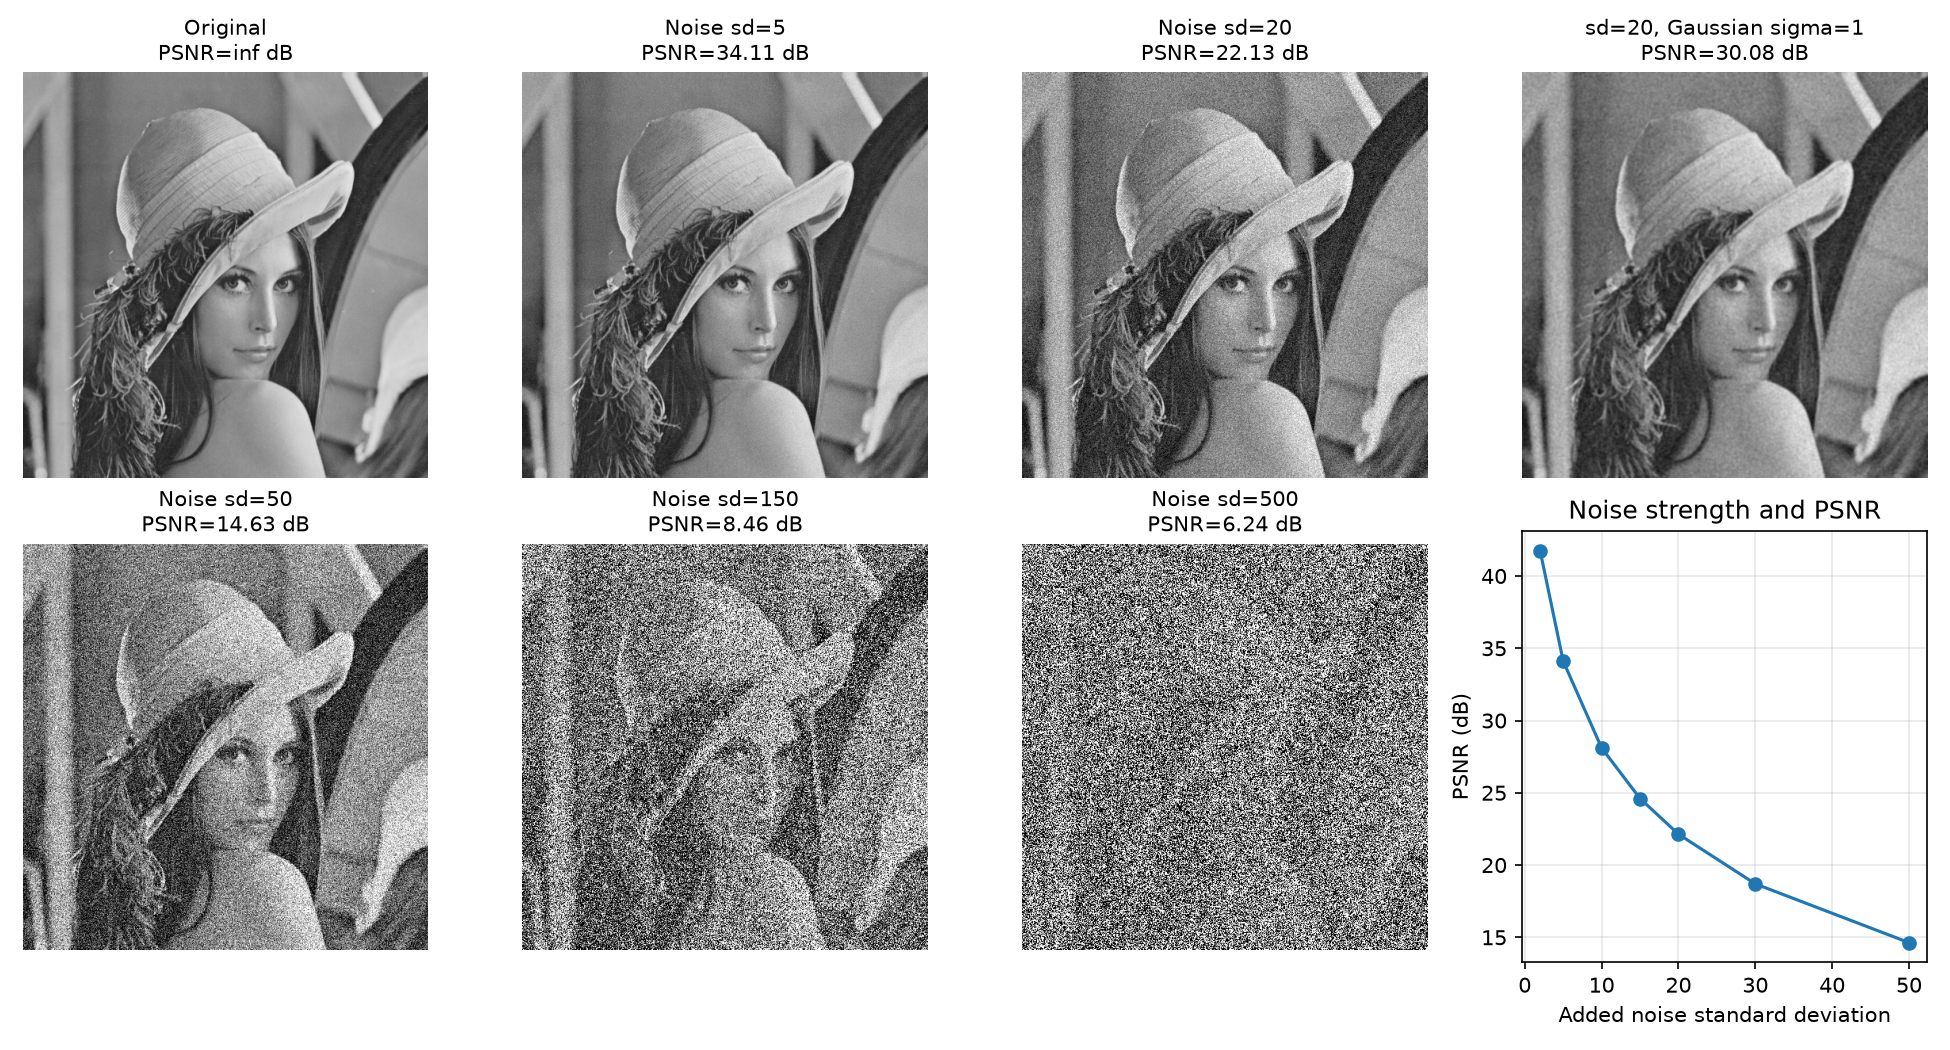
\includegraphics[trim=490.56bp 274.56bp 250.56bp 34.56bp,clip,width=\linewidth]{noise_filtering.png}
\end{minipage}\hfill
\begin{minipage}[b]{0.31\linewidth}
\centering\small Gaussian filter \(\sigma=1\)\\30.08 dB\\[2pt]
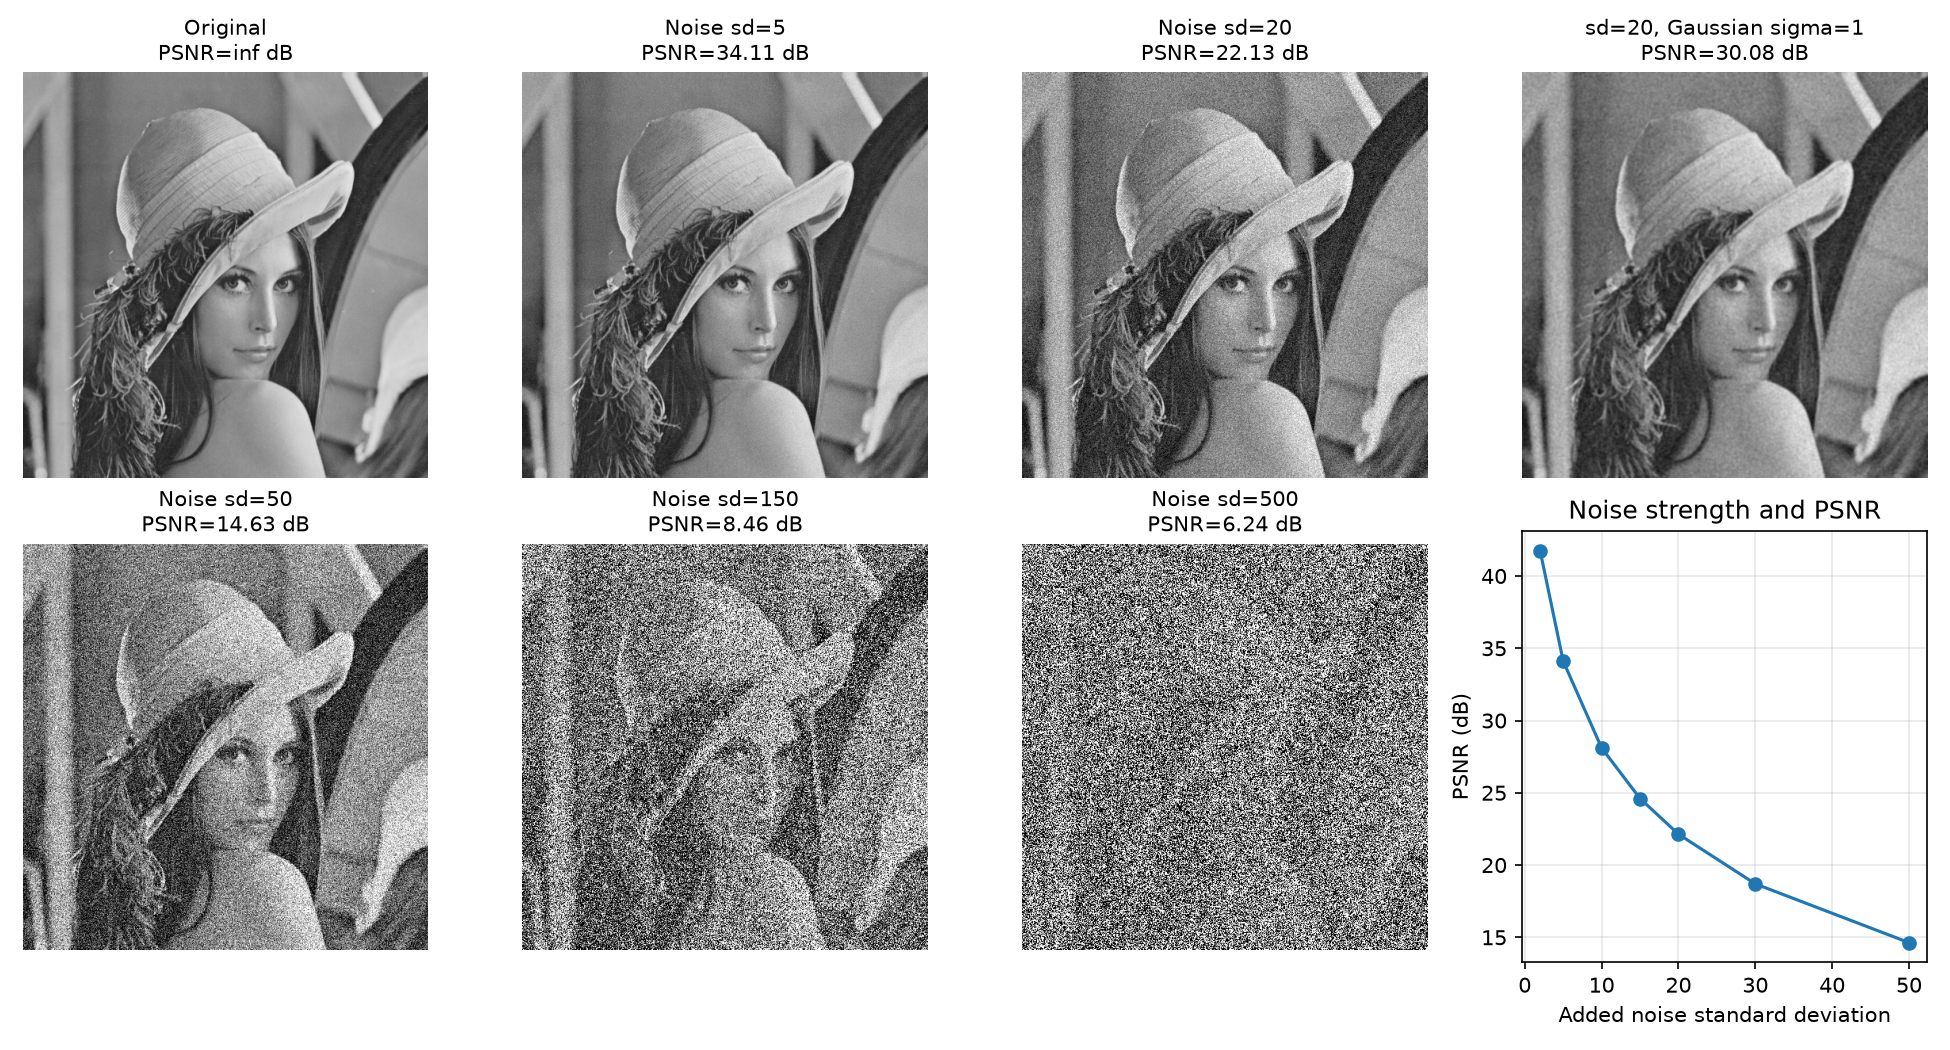
\includegraphics[trim=730.56bp 274.56bp 10.56bp 34.56bp,clip,width=\linewidth]{noise_filtering.png}
\end{minipage}\hfill
\begin{minipage}[b]{0.31\linewidth}
\centering\small Noise \(\sigma_n=500\)\\6.24 dB\\[2pt]
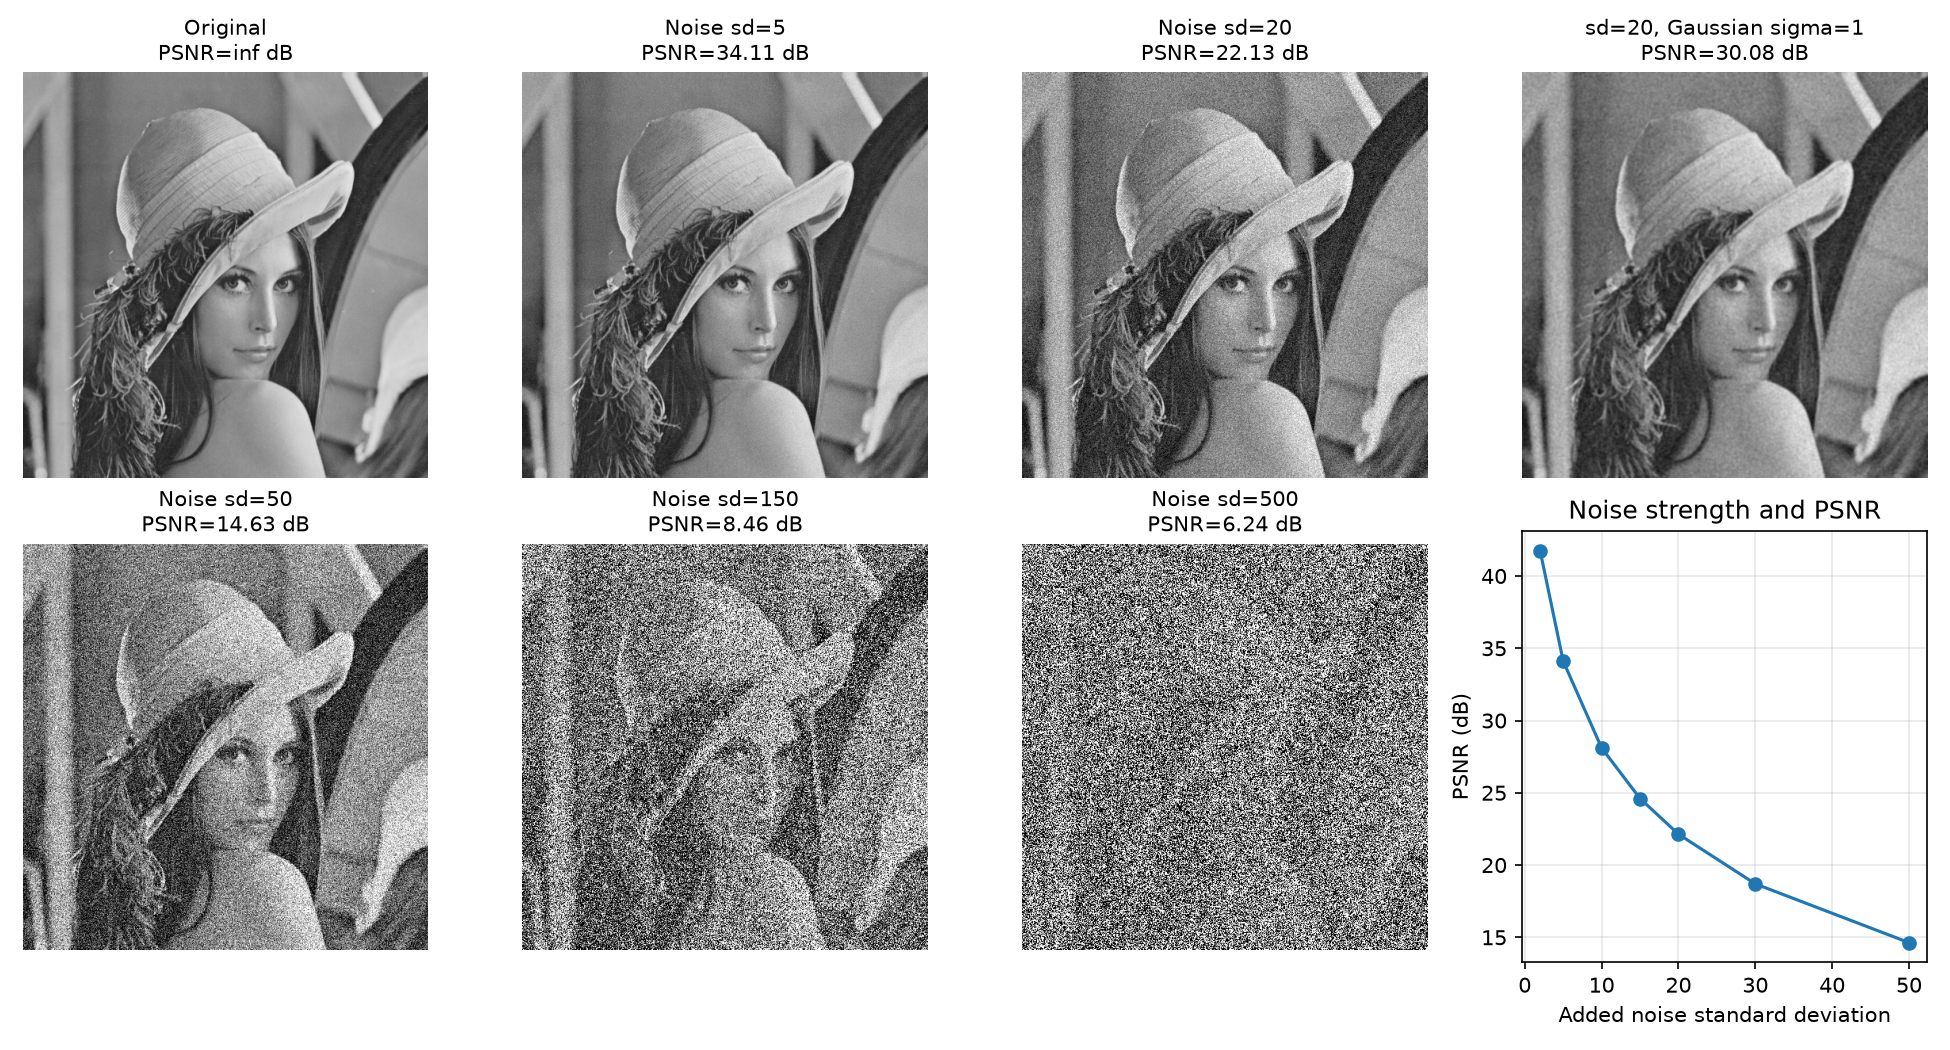
\includegraphics[trim=490.56bp 48bp 250.56bp 261.12bp,clip,width=\linewidth]{noise_filtering.png}
\end{minipage}
\caption{Noise before and after filtering, then severe noise. PSNR uses the clean original.}
\label{fig:noise}
\end{figure}

A more advanced method, Non-Local Means, averages similar image patches.
It can preserve texture and edges better than nearby averaging, but needs more
calculation and suitable settings
(\href{https://scikit-image.org/docs/stable/auto_examples/filters/plot_nonlocal_means.html}{scikit-image guide}).

% Teacher 3.1 Q1, Q2 and Q4; Q3, Q5 and Q6 continue on page 4.
\subsection{Audio Signal Analysis}
I loaded a
\href{https://raw.githubusercontent.com/parisjava/wav-piano-sound/master/wav/a1.wav}{piano note},
\href{https://www.pacdv.com/sounds/ambience_sounds/rain_2.wav}{rain} and
\href{https://www.pacdv.com/sounds/voices/can-you-keep-a-secret.wav}{speech}.
Stereo channels were averaged in floating point. Separate normalization means
the plots do not compare original loudness.

\begin{table}[H]
\centering
\caption{Audio measurements. The first three rows use complete clips.}
\label{tab:audio}
\small
\begin{tabular}{lrrrr}
\toprule
Clip & \shortstack{Sampling\\rate (Hz)} & \shortstack{Duration\\(s)} &
\shortstack{Strongest FFT\\peak (Hz)} & \shortstack{Highest bin\\at 1\% (Hz)}\\
\midrule
Piano & 44100 & 0.5018 & 219.21 & 4832.69\\
Rain & 22050 & 30.0301 & 272.56 & 11021.15\\
Speech & 44100 & 1.3013 & 290.48 & 15737.16\\
First 0.5 s speech & 44100 & 0.5000 & 290.00 & ---\\
\bottomrule
\end{tabular}
\end{table}

The highest-bin rule counts amplitudes at least 1\% of the strongest non-zero
frequency peak. Weaker components can extend higher, so this is not an exact
physical limit. The strongest peak is a separate measurement.

Piano showed fading regular oscillations, spectral peaks and harmonic bands.
Rain was less periodic with broad frequency content. Speech had bursts, gaps
and changing bands. Brighter regions mean greater power at that time and
frequency. No listening test was performed.

\begin{figure}[H]
\centering
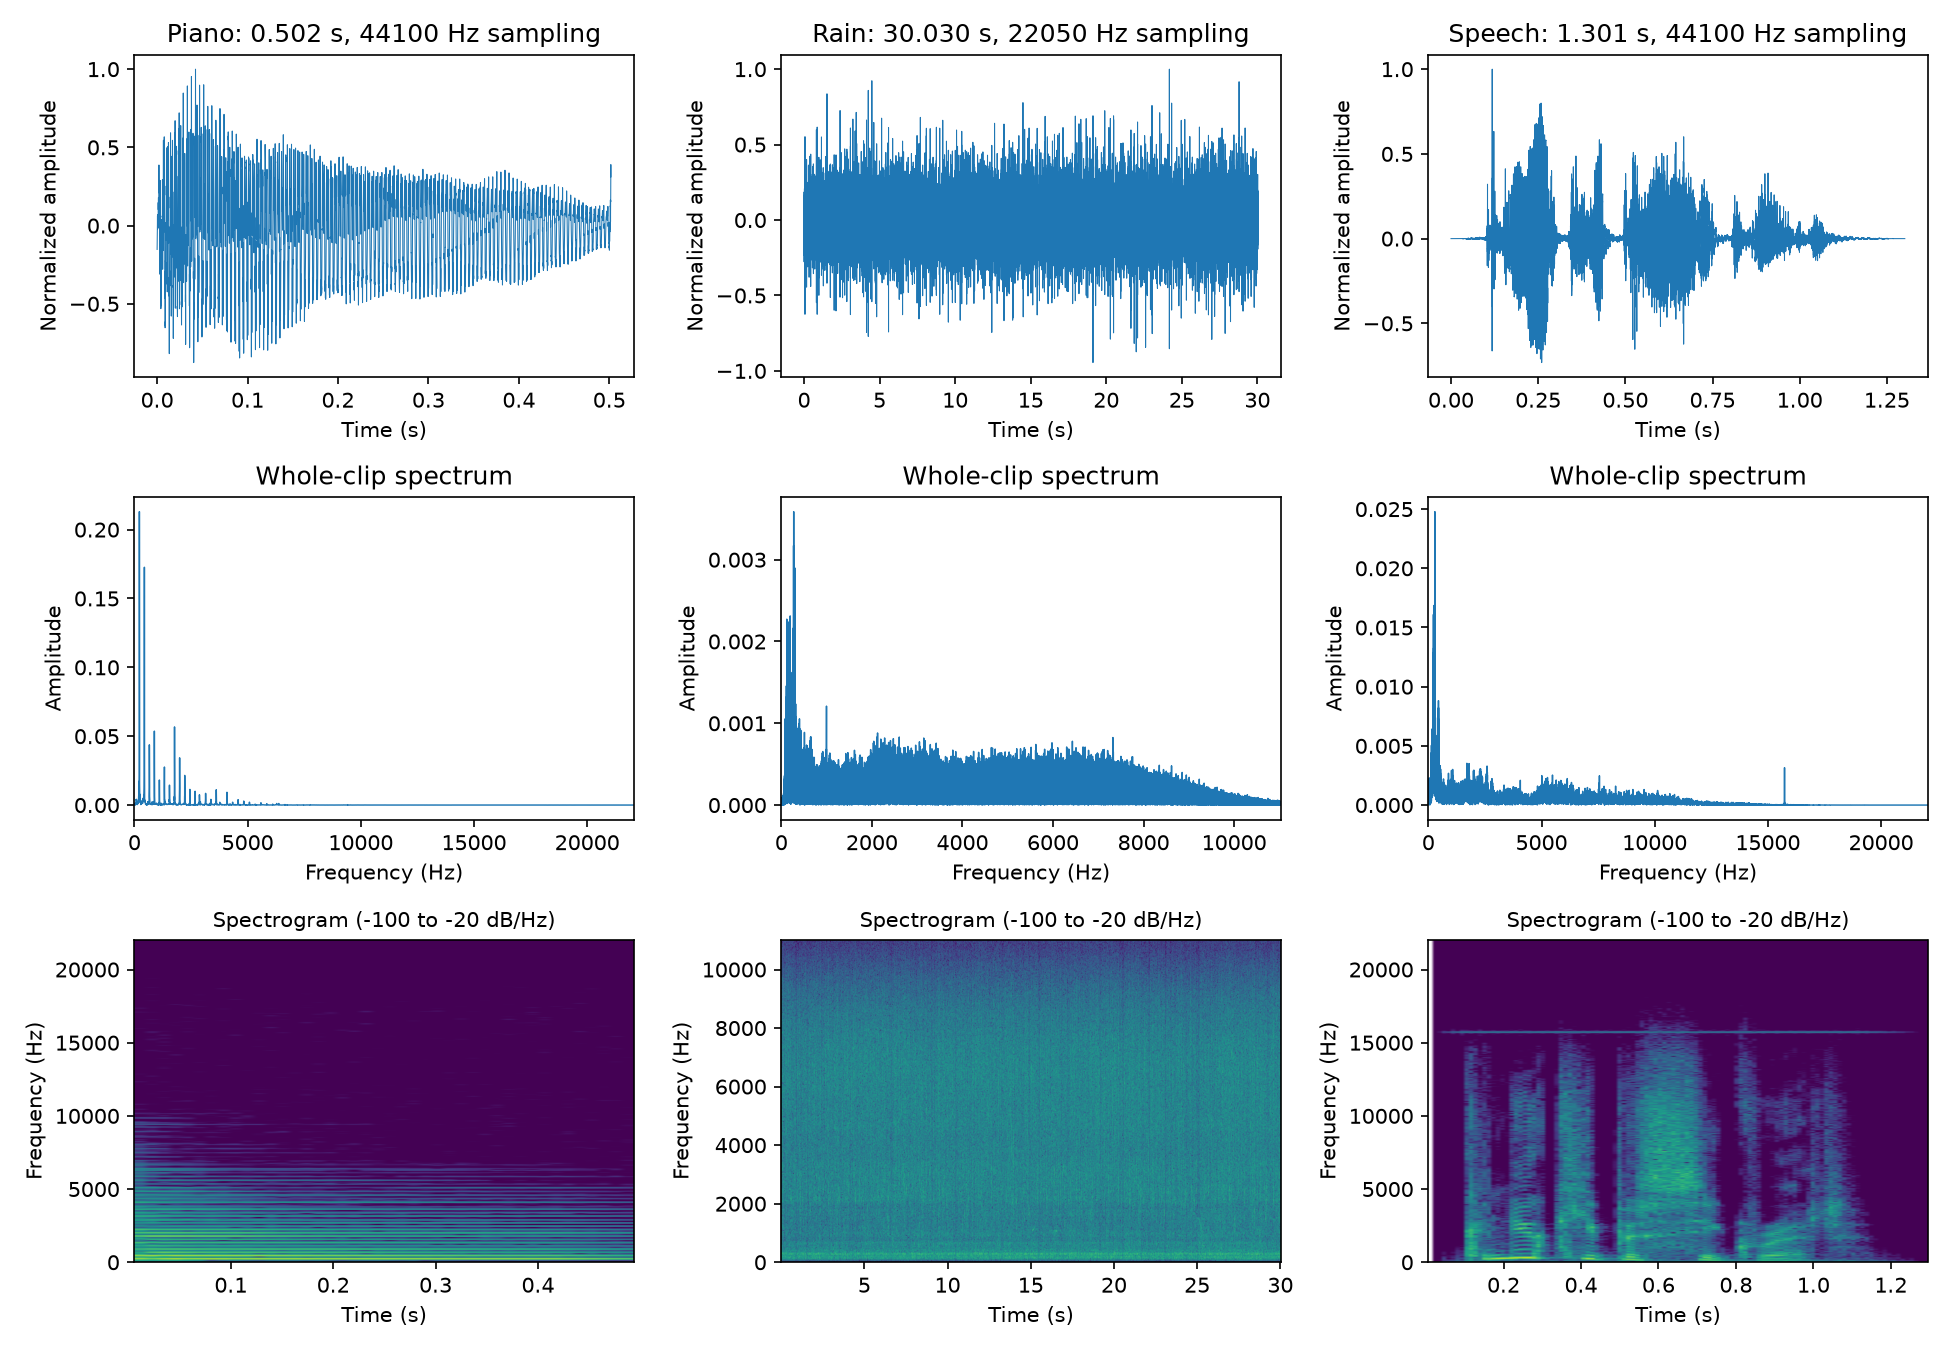
\includegraphics[trim=628.8bp 0 0 432bp,clip,width=100mm]{audio_types.png}
\caption{Speech: 1024-sample windows, 512-sample overlap. Power uses normalized amplitude.}
\label{fig:audio}
\end{figure}

% Teacher 3.1 Q3.
Cropping speech from 1.3013 s to 0.5 s kept 22050 samples. FFT spacing changed
from about 0.768 to 2 Hz. The main peak stayed near 290 Hz, but other strengths
changed because only the beginning was included. Both spectra used the same scale.

% Teacher 3.1 Q5.
Speech rates were 44100, 22050, 14700 and 7350 Hz. The waveform had fewer points
and the spectrum ended at the new Nyquist frequency. High frequencies folded
down because anti-alias filtering was omitted. The 2500 Hz tone stayed at
2500 Hz when sampled at 6000 Hz, became 1500 Hz at 4000 Hz sampling, and 500 Hz
at 2000 Hz sampling. Aliasing appeared below its 5000 Hz Nyquist rate;
this is not a listening threshold.

% Teacher 3.1 Q6.
Spectral noise reduction could estimate noise magnitudes from a quiet part,
reduce FFT magnitudes while keeping phases, and use an inverse FFT to return
to time samples. It may also damage quiet wanted sounds.

% The three concluding discussion questions.
\section{Discussion}
Sampling chooses time points for signals and audio, or pixel positions for
images. Quantization limits amplitude or grey levels. Too few samples can cause
aliasing; too few levels introduce rounding errors.

Images and audio share sampling, Fourier analysis and filtering, but images
have two spatial directions and mono audio one time direction. Communication
systems need suitable sampling, medical images need detail with controlled
noise, and multimedia balances data size against picture and sound quality.

\section{Conclusion}
The lab showed how sampling, quantization and noise change represented
information. FFT analysis exposed frequency content and aliasing. Quality
measurements helped compare results, while visual observations showed their limits.

\section*{Appendix: Code Snippets}
\small
\textbf{A. Chirp generation.} The sweep duration sets how quickly frequency changes.
\lstinputlisting[firstline=116,lastline=119]{../signals.py}

\textbf{B. PSNR calculation.} Converting to float before subtraction prevents 8-bit wraparound.
\lstinputlisting[firstline=53,lastline=59]{../images.py}

\textbf{C. Audio downsampling.} Keeps every nth sample and lowers its rate.
Filtering was omitted to show aliasing.
\lstinputlisting[firstline=120,lastline=121]{../audio.py}
\end{document}
